\chapter{Colorization}
\label{chapterlabel3}

Colorization is the process of adding plausible colors to monochrome images, it is a highly uncertain problem that has not a unique solution. In the context of this master project, we are interested in anime-style sketch colorization, a few distinctive characteristics includes:

\begin{itemize}
    \item Unlike grayscale image input, its input is a binary sketch image.
    \item Unlike realistic image colorization, the output is heavily style-oriented, has less well-defined details, and therefore comparably nondeterministic nature.
    \item Unlike many colorization researches, the task of filling missing regions is not assessed. The full sketch image is provided without cropping.
    \item It is relatively difficult to find a dataset that contains large amount of high quality pairs of sketch and colorized anime image, because artists often do not include it when uploading to the internet.
\end{itemize}


\section{Approaches \& Methods}
Anime-style sketch colorization is a sub-field in image-to-image translation task. It is a difficult problem because there are infinite number of ways to produce feasible results, therefore color strokes are often given as additional input to hint the model to output in a certain style (user-guided colorization). There are many attempts to this problem and I will introduce them in the following paragraphs.

Traditional computer assisted colorization uses an algorithmic approach. Typically, the user first crops the region that he/she wants to color, then apply a color scheme from a palette, finally the computer will run an algorithm to perform colorization. A popular approach is to minimize the difference between a pixel's color and its weighted average of neighbouring pixels' colors.\cite{levinColorizationUsingOptimizationb} The intuitive is neighboring pixels with similar intensity should have similar colors. This method generates high quality results, but it is time consuming because it requires detailed color input and manual cropping. Follow up researches attempted to reduce the effort via learning-based methods, such as interpolation of user-drawn scribbles using boosting \cite{liScribbleBoostAddingClassification2008} or manifold learning \cite{chenManifoldPreservingEdit2012}; and determine the importance of image feature automatically using neural network \cite{endoDeepPropExtractingDeep2016}.


\begin{figure}
    \centering
    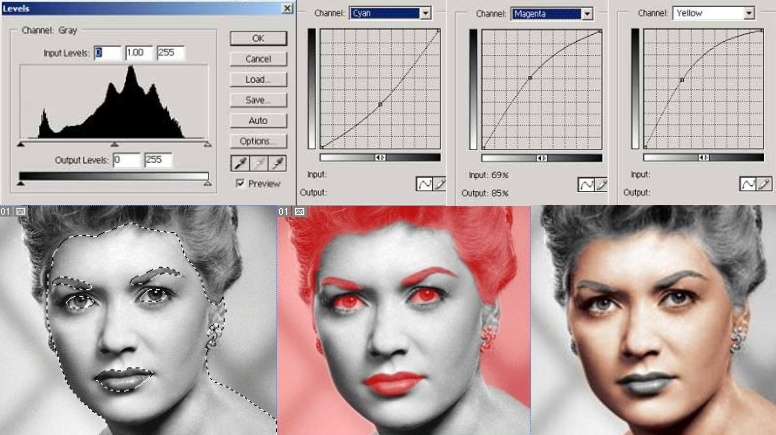
\includegraphics[width=0.75\textwidth]{images/colorization/computer_assisted_colorization.jpg}
    \caption{Example interface for traditional computer assisted algorithmic colorization. Top shows an interface for selecting a color; bottom-left and bottom-middle show interfaces for selecting a region; and bottom-right shows the resulting image.\cite{ColorizeBlackWhite}}
    \label{fig:computer_assisted_colorization}
\end{figure}

While these methods introduced remarkable improvements, image colorization remains a time-consuming task. In addition, traditional methods often make use of intensity information which does not presents in anime sketches, which made them unsuitable. In recent years, machine learning based methods started to gain popularity as availability of computing resource increases. The milestone work of Pix2pix\cite{isolaImagetoImageTranslationConditional2018} demonstrated a simple yet general architecture for image-to-image translation task. It outperforms vanilla CNN by a large margin (see figure \ref{fig:colorization_cnn} for vanilla CNN outputs) However, directly apply Pix2pix model will result in artifacts such as \textit{color bleeding}\footnote{Color overflows boundaries defined by sketches.} and \textit{dirtiness}\footnote{Abrupt smoky color patches that are not defined by the sketches.}, they result in inconsistency and unpleasing colorization (see figure \ref{fig:colorization_pix2pix} for Pix2pix outputs). 

\begin{figure}
    \centering
    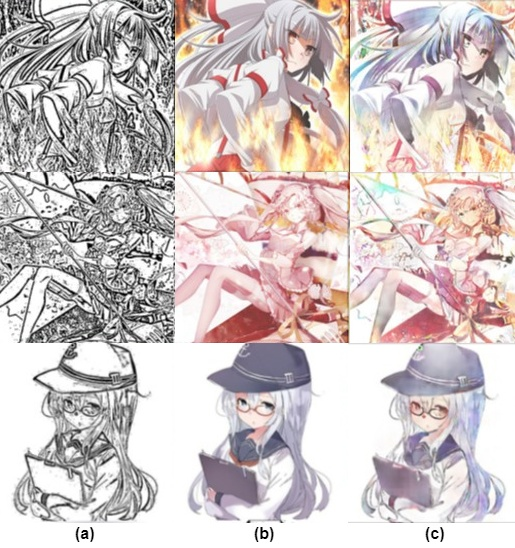
\includegraphics[width=0.75\textwidth]{images/colorization/cnn.jpg}
    \caption{Vanilla CNN output for anime sketch colorization. Column (a) is the input sketches; column (b) is the target image; and column (c) is the output image.\cite{fransOutlineColorizationTandem2017} We can see that the output suffers from a number of obvious issues, such as random fading and dirty colors, and obvious convolutional artifacts. It is far from visually pleasing.} 
    \label{fig:colorization_cnn}
\end{figure}

\begin{figure}
    \centering
    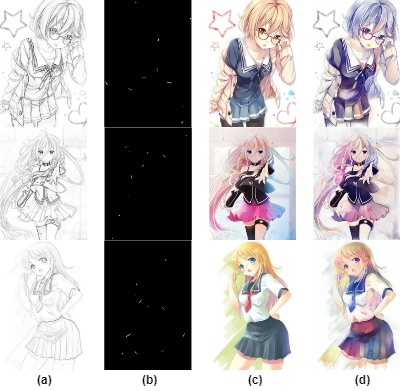
\includegraphics[width=0.85\textwidth]{images/colorization/pix2pix.jpg}
    \caption{Vanilla Pix2pix output for anime sketch colorization. Column (a) is the input sketches; column (b) is the color hint; column (c) is the target image; and column (d) is the output image.\cite{steinsDeepLearningProject2022} The coloring are reasonable but suffer from artifacts such as color bleeding and has a certain degree of dirtiness. For example, the colors are different in each stripe of the skirt. But we can also observe that the color is more coherent than the vanilla CNN models as less convolution artifacts are produced.} 
    \label{fig:colorization_pix2pix}
\end{figure}

PetalicaPaint\cite{PetalicaPaint} used a doubly linked deep U-Net architecture to address style inconsistency problem, by having a deeper network, the model is able to capture the general distribution and keep it consistent. However, it's style varies on loss function hyper-parameters which means each model can only paint with one style (see figure \ref{fig:colorization_petalica}).

\begin{figure}
    \centering
    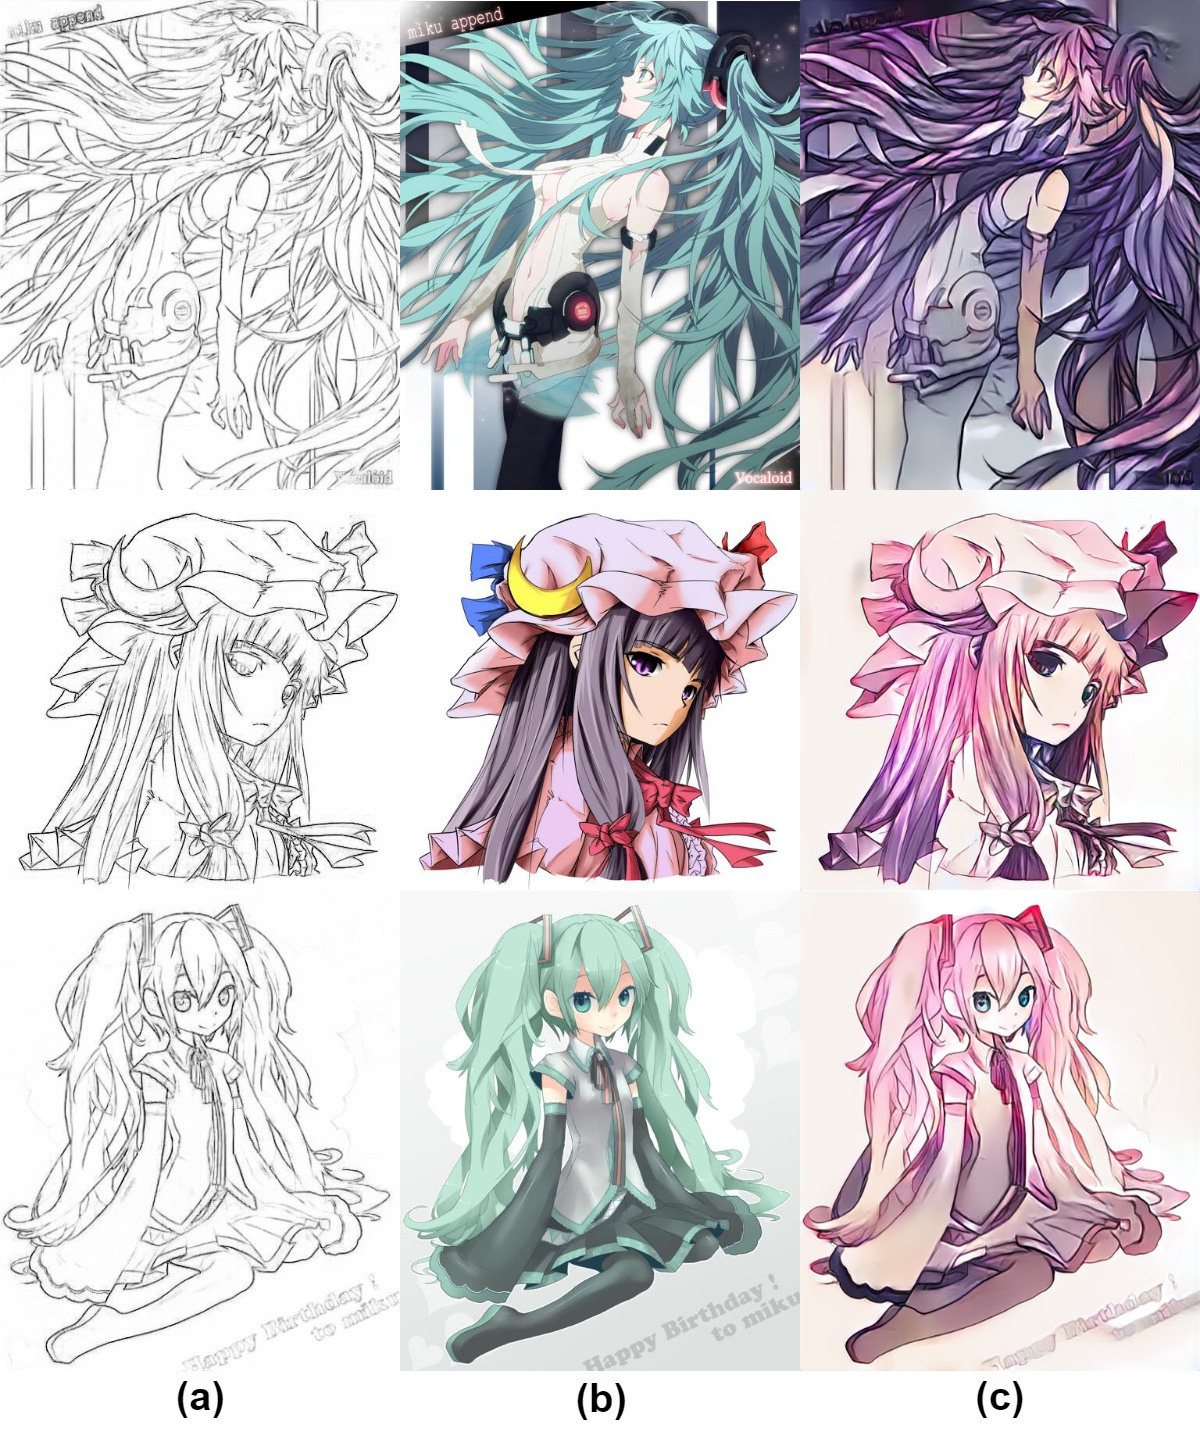
\includegraphics[width=0.75\textwidth]{images/colorization/petalica.jpg}
    \caption{Petalica Paint output for anime sketch colorization, painted with \textit{Canna\protect\footnotemark}  style. Column (a) is the input sketches; column (b) is the target image; and column (c) is the output image.\cite{steinsDeepLearningProject2022} The coloring showed consistency across different region with clean and pleasible coloring with local shading, however, there is little artistic texture and global shading presents in the colored image.} 
    \label{fig:colorization_petalica}
\end{figure}

\footnotetext{The name of the style given to a particular model by the author.}

Although the result is much more pleasing, it is still not as vivid as most colored image, two most obvious features missing are artistic texture and global shading. Artistic texture allows the model to have slightly different styles in different region of the image and global shading allows the model to draw sensible shadows and highlights. Fortunately, follow up researches showed that we can obtain artistic texture by using content loss and obtain global shading simply by increasing the receptive field of the U-Net block's decoders\cite{ciUserGuidedDeepAnime2018}. This is the AlacGAN model, which I will explain in details below, sample output can be found at figure \ref{fig:colorization_alacgan}.

\begin{figure}
    \centering
    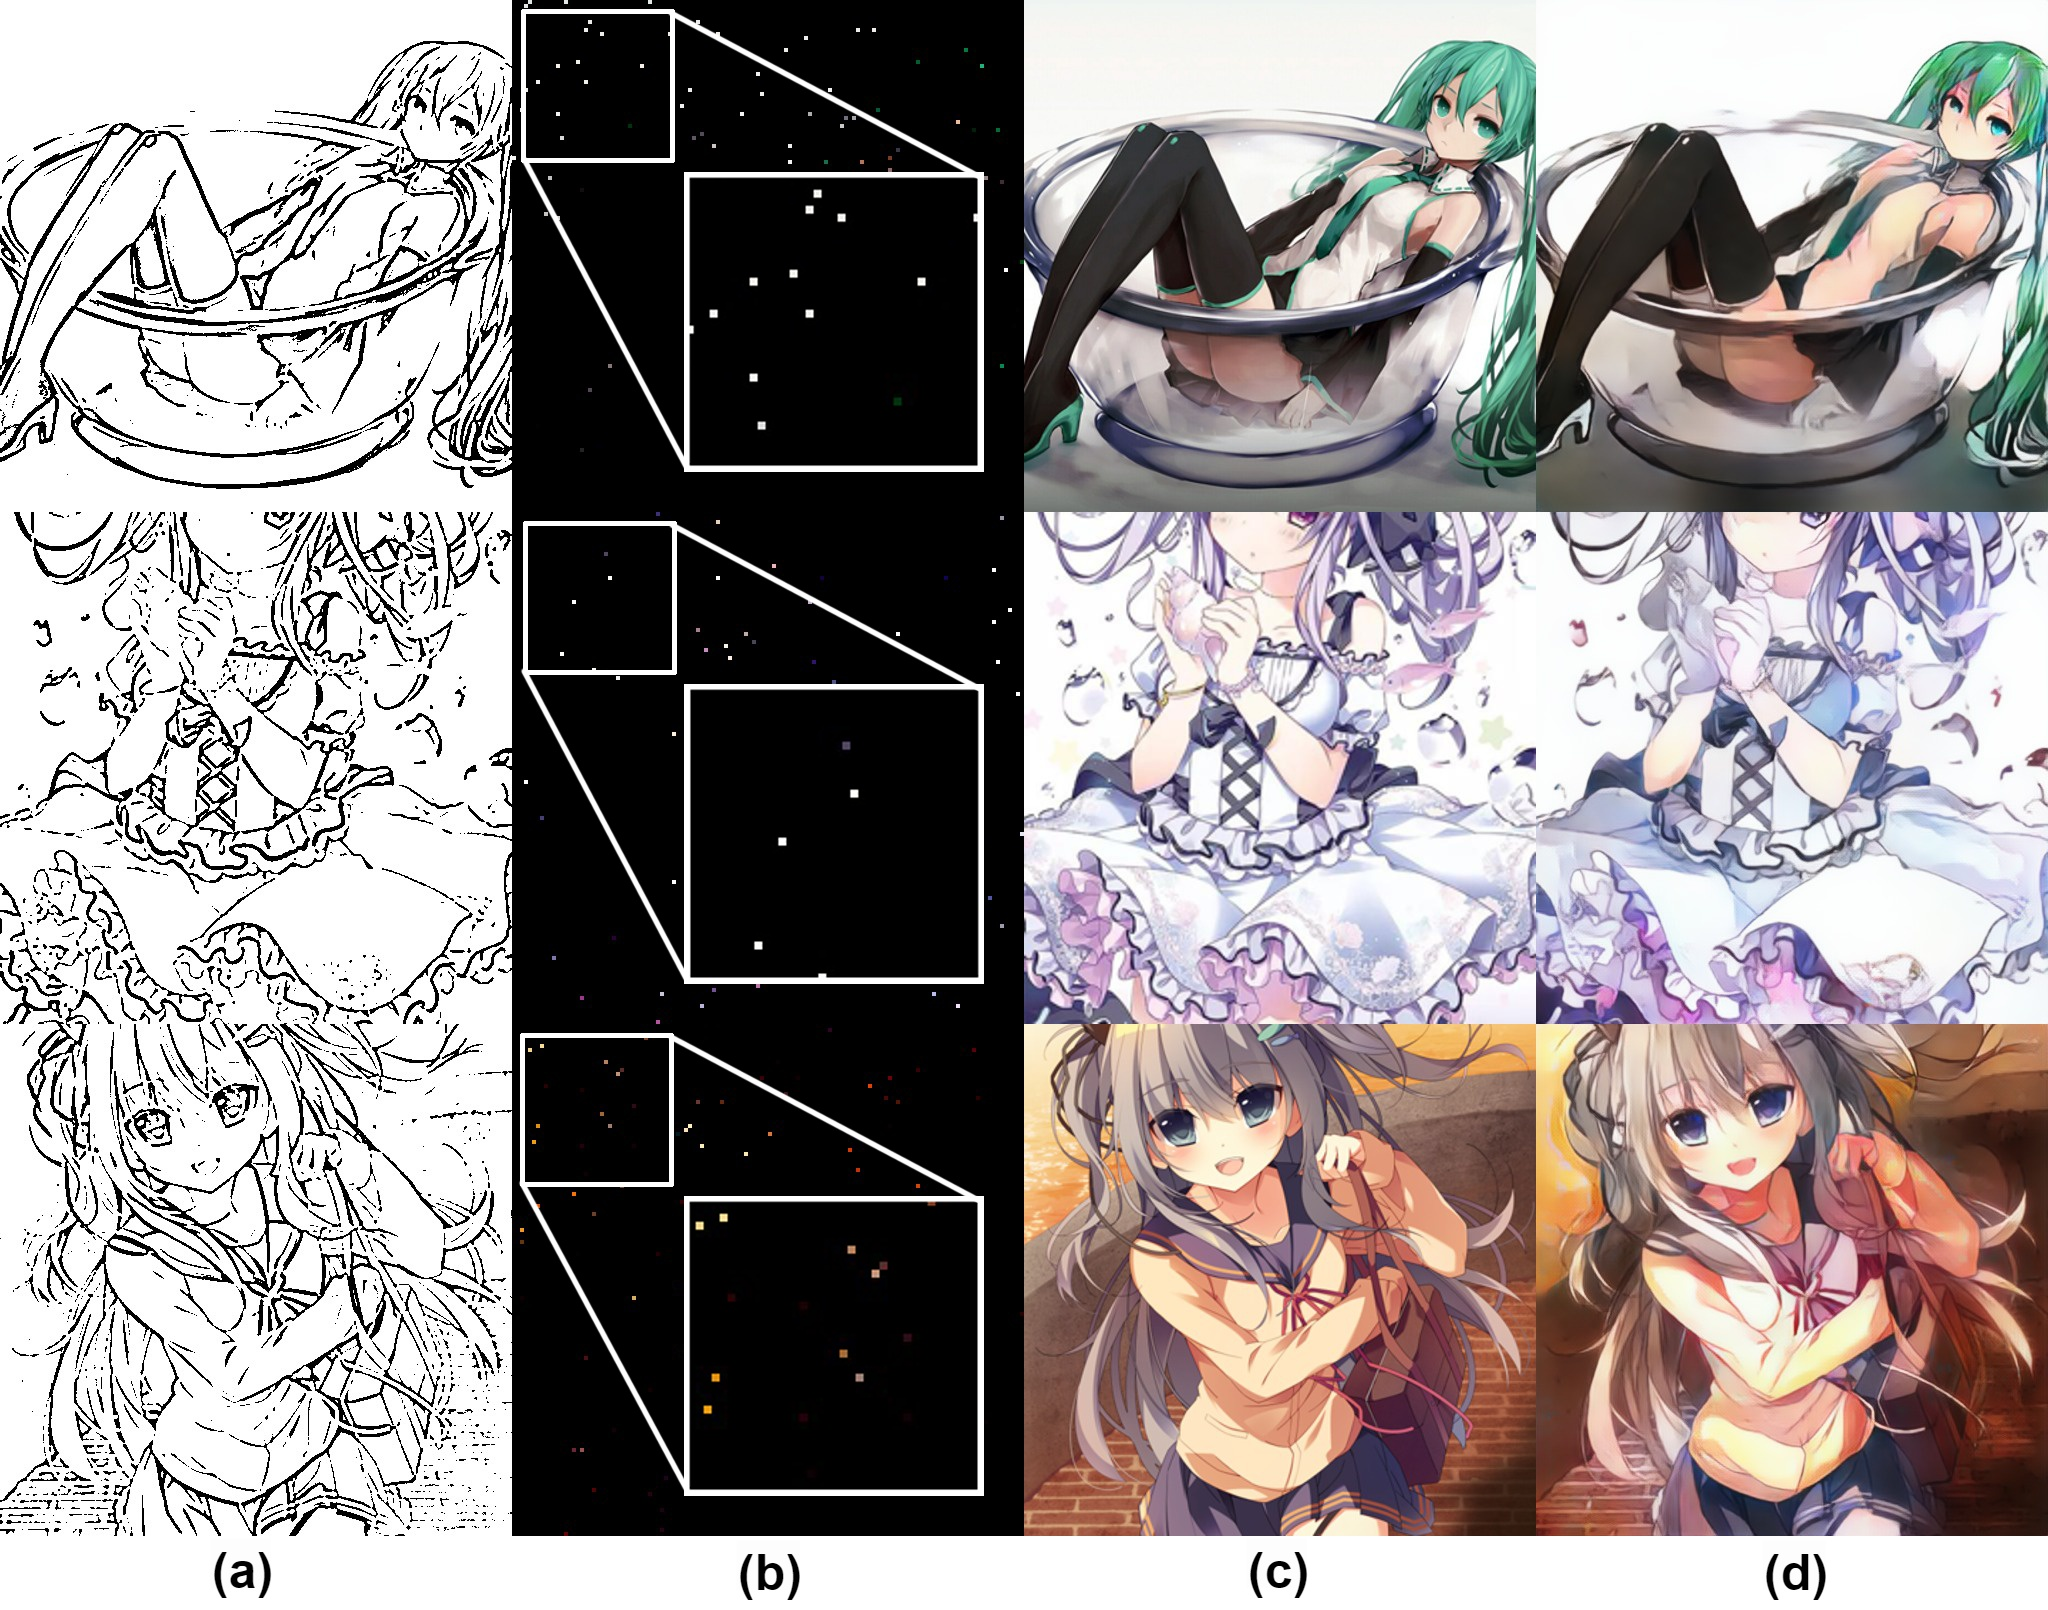
\includegraphics[width=0.85\textwidth]{images/colorization/alacgan.jpg}
    \caption{AlacGAN output for anime sketch colorization. Column (a) is the input sketches; column (b) is the color hint, the white box enlarges a part of the hint for ease of viewing sample points; column (c) is the target image; and column (d) is the output image. We can observe that the present of global shading and diverse artistic textures result in a much more vivid output.}
    \label{fig:colorization_alacgan}
    %\todo[inline]{enlarge part of the hint so that they are easier to see.}
\end{figure}

\section{Design \& Implementation}

\subsection{Dataset}
The input the model is a binary anime sketches and output is the colorized version of the sketch. It is difficult to find a large amount of such pairs, most researches generates sketches from colored image. Real world anime arts contains a large variety of contents, and thus as a pretrain model, our dataset should cover as much styles as possible to ensure its generality. Popular large illustration dataset such as Nico-opendata\cite{Undefineda} and Danbooru\cite{branwenDanbooru2021LargeScaleCrowdsourced2015} are not suitable because it contains many scribbles, result in hard to clean noise. Therefore I adopted the dataset from the original paper, which is crawled from the internet by the authors.

\subsection{Model}

% Tobias says he does not care about architecture 
% \begin{figure}
%     \centering
%     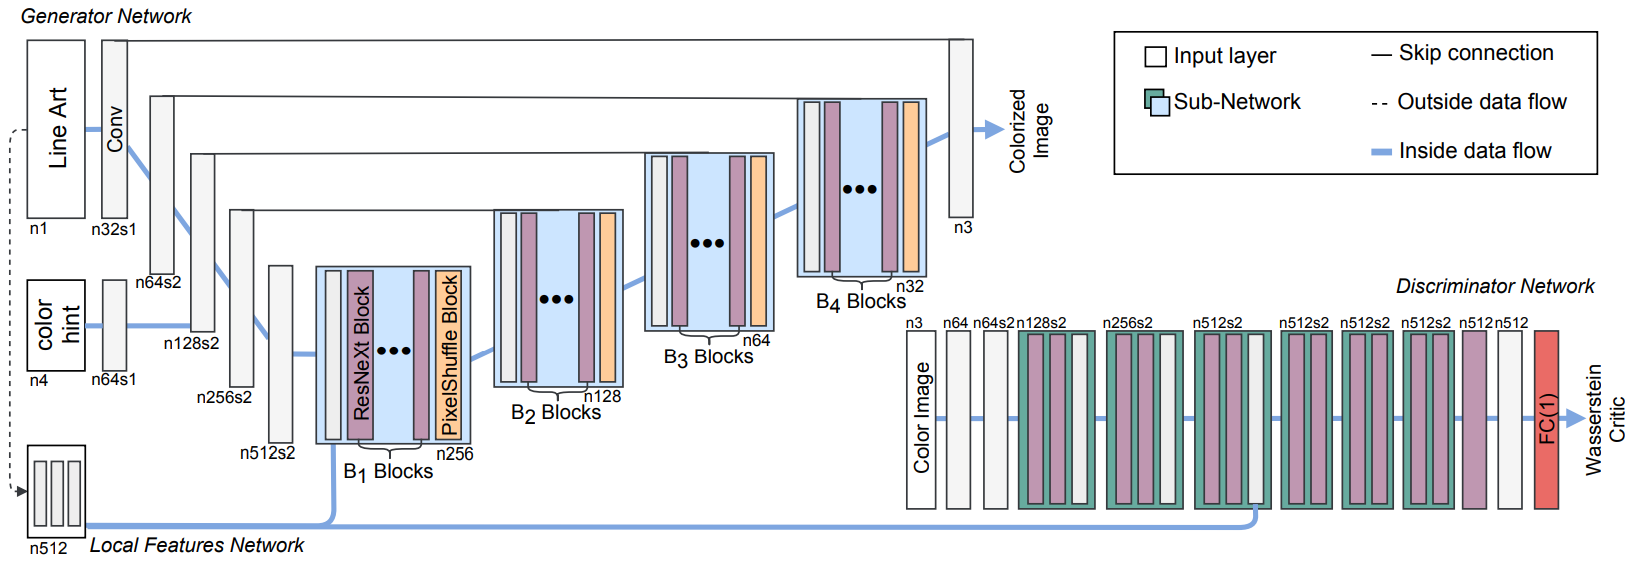
\includegraphics[width=1.0\textwidth]{images/colorization/alacgan_arch.png}
%     \caption{Architecture of Generator and Discriminator Network with corresponding number of feature maps (n) and stride (s) indicated for each convolution block.} 
%     \label{fig:alacgan_arch}
% \end{figure}

The model follows a GAN architecture, including a generator $\mathcal{G}$ and a discriminator $\mathcal{D}$. The generator employs an U-Net\cite{ronnebergerUNetConvolutionalNetworks2015} architecture.
%Figure \ref{fig:alacgan_arch} shows the overall structure of the model.

The generator convert both the sketch and color hint to feature map and repeatedly convoluted and half-scaled them until the features are same size as the local feature network output. The local feature network is a pretrained network that extract feature from the input sketch. Then both outputs are concatenated and repeatedly double-upscale using sequential ResNeXt tunnel until the original dimension. The ResNeXt tunnel is a sequential stack of ResNeXt block\cite{xieAggregatedResidualTransformations2017a} with a pixelshuffle block\cite{shiRealTimeSingleImage2016} appended at the end. It uses ResNeXt block because it is more effective for increasing capacity compared to the vanilla resnet block without additional computational cost. Normalization layer is not used because it reduces flexibility for accurate colorization\cite{nahDeepMultiscaleConvolutional2018}.

The discriminator takes the concatenation of sketch features and colored image as input, forming a cGAN\cite{mirzaConditionalGenerativeAdversarial2014} and employ a SRGAN\cite{ledigPhotoRealisticSingleImage2017} architecture without dilation as we do not need to upscale the image like the original paper does.

The local features are extracted from the sketch image using a pretrained feature extraction network $\mathcal{F}1$. They contains both semantic and spatial information of the sketch. This helps to reduce overfitting on synthetic sketch because human drawn sketches can be very different from synthetic sketches, but the local feature network is pretrained on human drawn illustration which will not affect by synthetic lines. Specifically, the $6^{th}$ convolution layer of the Illustration2Vec\cite{saitoIllustration2VecSemanticVector2015} network is used. It is pretrained on 1,287,596 illustrations, including sketches and colored images, predicting 1,539 labels.

The hint $H$ is randomly sampled pixels from the colored image, the hint has the size 1/4 of the colored image.

The second feature extractor $\mathcal{F}2$ is used to compute the content loss of the fake and real colored image. It is the $4^{th}$ layer of the VGG16 network, pretrained on ImageNet\cite{ImageNet}.

\begin{figure}
    \centering
    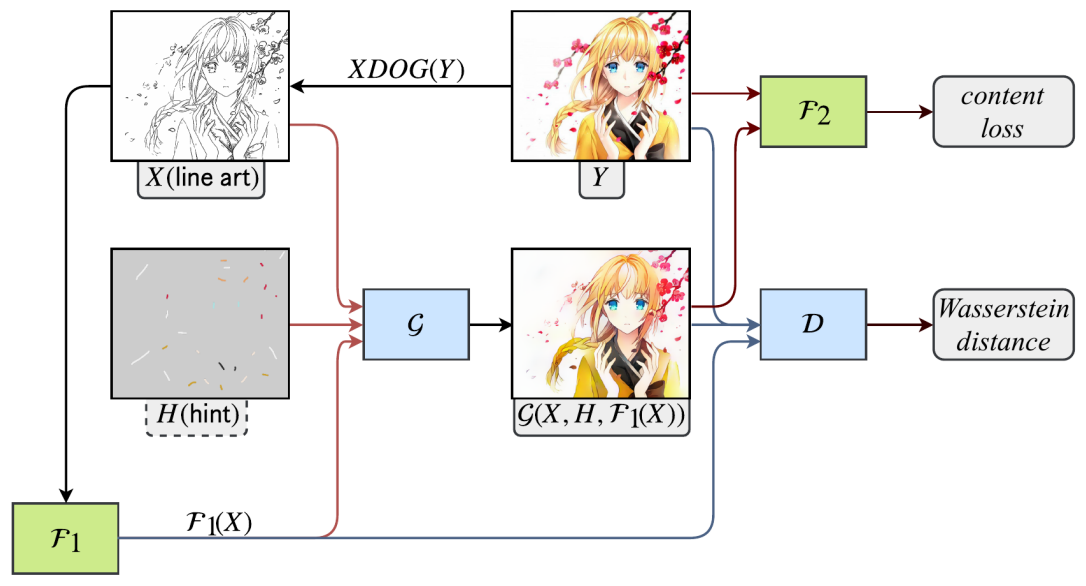
\includegraphics[width=0.75\textwidth]{images/colorization/alacgan_train.png}
    \caption{Overview of training process of AlacGAN Network. $\mathcal{F}1$ and $\mathcal{F}2$ denotes two pretrained feature extractors; $\mathcal{G}$ denotes generator and $\mathcal{D}$ denotes discriminator; $X$ denotes input sketch; $H$ denotes optional input color hint; $Y$ denotes target colored image and XDOG denotes the sketch generated from the colored image.} 
    \label{fig:alacgan_train}
\end{figure}

\begin{figure}
    \centering
    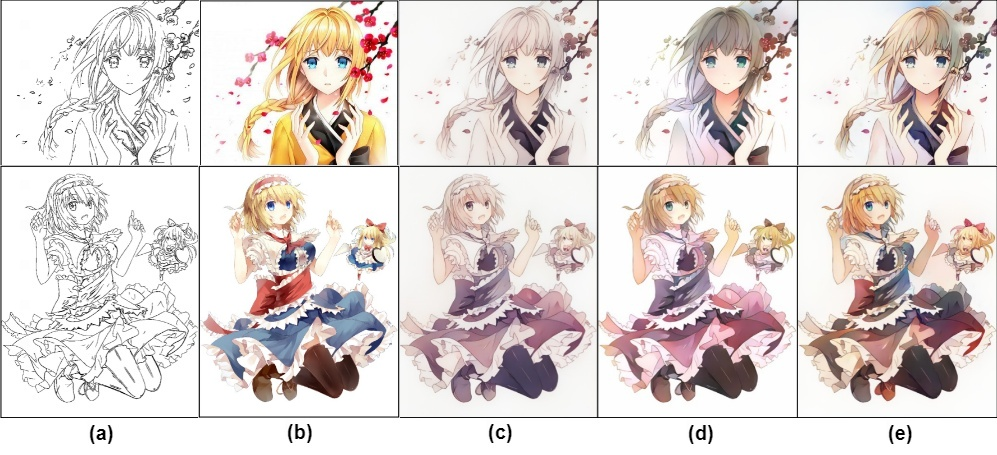
\includegraphics[width=1.0\textwidth]{images/colorization/alacgan_features.jpg}
    \caption{Comparison of different techniques used in AlacGAN. (a) denotes input sketch; (b) denotes the target output; (c) denotes output without adversarial loss; (d) denotes output without local feature network; and (e) denotes output when both exists. We can see that when adversarial loss is missing, color can be diluted. When local features network is missing, global shading can be absent. When both techniques are used, the result looks much more vivid and closer to target image.} 
    \label{fig:alacgan_features}
\end{figure}

\subsection{Preprocessing}
For each colored image collected, I used the XDoG\cite{winnemollerXDoGEXtendedDifferenceofGaussians2012} algorithm to generate synthetic sketches that stimulate real sketch drawings. The settings are sigma = $0.3/0.4/0.5$; k sigma = $4.5$; epsilon = $0$; phi = $10\mathrm{e}9$; and gamma = $0.95$. Different sigmas are randomly chosen during training to stimulate different stroke thickness. During preprocessing, all three different sigmas images are generated beforehand to speed up training. All images are also crop and resized to $512\times512$.
\todo[inline]{Add more details}

\subsection{Training}
I pretrained with the following settings, similar to the original paper: batch size=8, epoch=500, optimizer=Adam, optimizer betas=(0.5, 0.999), learning rate=0.0001, scheduler=step, scheduler step size=400, scheduler gamma=0.1. The dataset contains 20k images, split for training and testing with ratio 9:1.

As for data augmentation, random resized crop, random jittering and random horizontal flip are applied to improve model's generalization capability. After augmentation, images are also normalized with mean and variance of $0.5$ for more stabilized input.

\todo[inline]{Show NoGhost result}

\section{Future Direction}
While AlacGAN is able to produce results with global shading and artistic texture, there are still rooms for improvement. First of all, although the model is able to generate colored image according to color hint input, there are little control over other aspects of the output. For example, the direction of light and color tones. In the context of this master project, keeping the same object the same color and styles constant across hundreds of frames or even in another scene can be a challenging task.

As the most challenging task in this master project, the final AlacGAN model generates colored images at 1 frame per second (FPS). It is expected to be the bottleneck of the whole pipeline. To improve the speed of the inference, we can attempt the following ideas:

\begin{itemize}
    \item \textbf{Knowledge distillation} The pretrained local feature network can be useful at time but it can be computational expensive and utilized at max capacity. We can introduce a smaller feature network and uses the pretrain local feature network as the teacher to guide its learning. This processing is known as knowledge distillation (see appendix \ref{app:ml:kd}). This idea can be expanded to other parts of the network to further compress the model.
    \item \textbf{Domain specific tuning} The current model is pretrained with thousands of online images, each of them are colored individually with detailed styling and artistic details. However, it is uncommon for 2D animation to achieve such level of details. By observing the frames from NoGhost, it is obvious that the most common coloring technique used is flat shading with little color variation within the same enclosed region. Therefore, we could potentially reduce the receptive field of the ResNeXt convolution tunnels to achieve similar results.
\end{itemize}

